\documentclass[onecolumn]{article}
\usepackage[spanish]{babel}
\usepackage{caption}
\usepackage{graphicx}
\usepackage{amsmath}
\setlength{\parindent}{0pt}

\author{Josué Villasante}
\title{Espectroscopia gamma utilizando detectores de NaI, HPGe y BGO}

\begin{document}
	\maketitle
	\begin{abstract}
		testing
		${}^1_2X^3_4$
	\end{abstract}

	\section{Introducción}
	
	\section{Materiales y método}
		Se utilizó el simulador Radess. En este no es posible controlar el voltaje de la fuente de alto voltaje, ni la ganancia dada por el amplificador. Por lo tanto, estos no se modificaron. La fuente de alto voltaje se mantuvo constante en 900 voltios.

	\section{Resultados}	
		Se realizó la calibración para cada detector. Se trabajo con los siguientes: NaI3x3, HPGe y BGO. Para cada uno se realizó una calibración utilizando diversos isótopos considerando su energía. Estos están incluidos en la tabla \ref{table_energies}.

		\begin{center}
			{\renewcommand{\arraystretch}{1.5}
			\renewcommand{\tabcolsep}{0.2cm}
			\captionof{table}{Isotipos utlizados en la calibración y sus energías}
			\label{table_energies}
			\begin{tabular}{ c c c }
				\hline
				Isótopo & Probabilidad(\%) & Energía (keV) \\
				\hline
				${}^{137}\mathrm{Cs}$ & 85 & 662 \\ 
				${}^{22}\mathrm{Na}$ & 180 & 511 \\ 
				${}^{22}\mathrm{Na}$ & 100 & 1275 \\ 
				${}^{60}\mathrm{Co}$ & 99 & 1173 \\ 
				${}^{60}\mathrm{Co}$ & 100 & 1332
			\end{tabular}}
		\end{center}

		Primero se obtuvieron los resultados para el detector de NaI3x3. Para todos las fuentes se configuró una actividad de $10^5$Bq y se realizó la medición por 5 segundos a una distancia de 1cm. La única excepción fue para el ${}^{60}\mathrm{Co}$. Su medición se realizó por 15 segundos.

		\begin{center}
			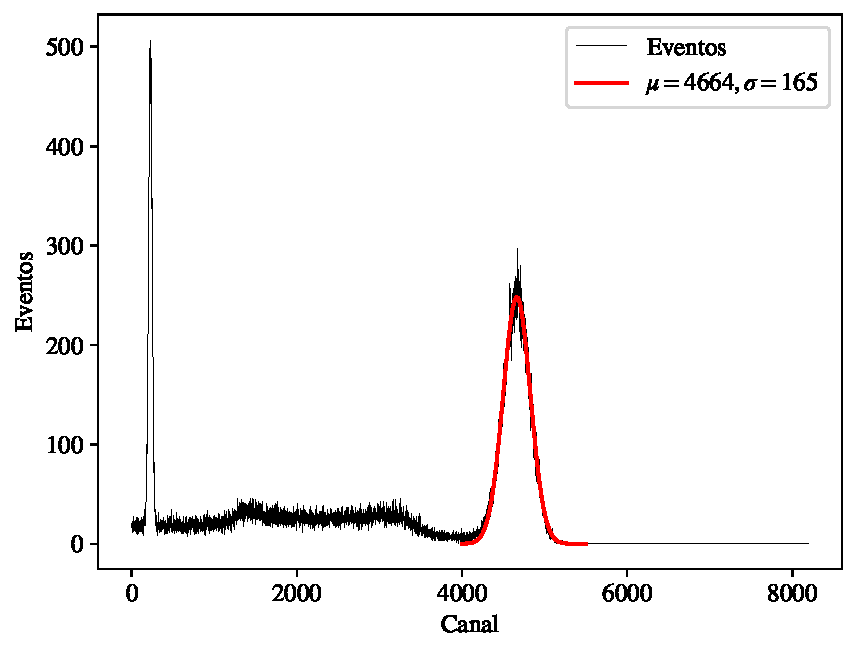
\includegraphics[width=225pt]{img/nai_33_cs_137.pdf}
			\captionof{figure}{Espectro de una fuente de ${}^{137}\mathrm{Cs}$ y su ajuste}
		\end{center}

		\begin{center}
			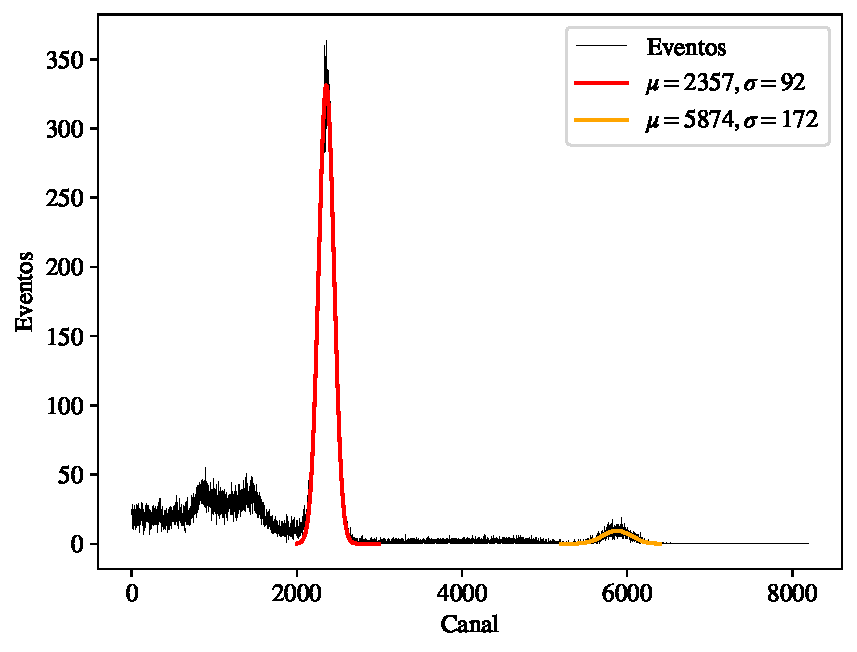
\includegraphics[width=225pt]{img/nai_33_na_22.pdf}
			\captionof{figure}{Espectro de una fuente de ${}^{22}\mathrm{Na}$ y su ajuste}
		\end{center}

		\begin{center}
			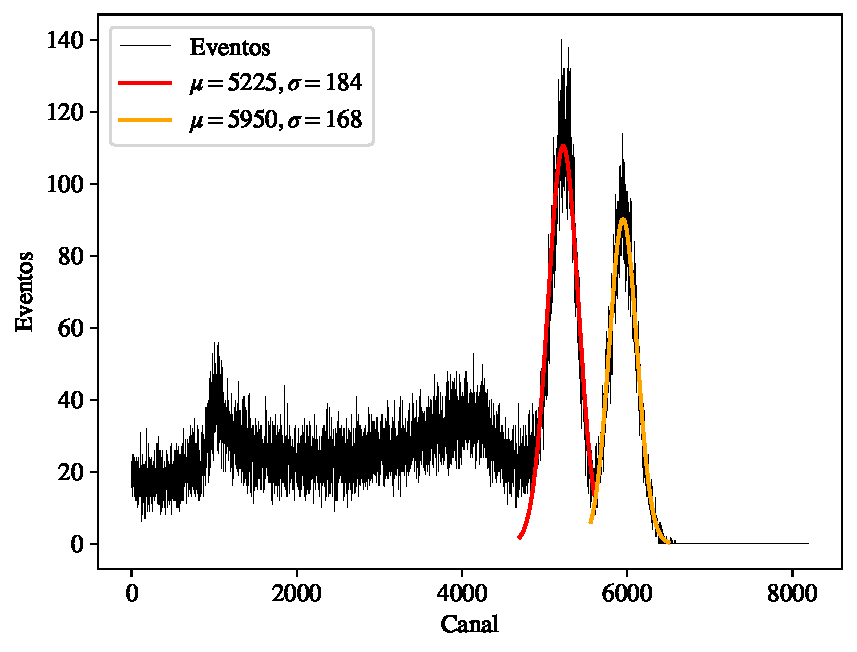
\includegraphics[width=225pt]{img/nai_33_co_60.pdf}
			\captionof{figure}{Espectro de una fuente de ${}^{60}\mathrm{Co}$ y su ajuste}
		\end{center}

		Luego se obtuvieron los resultados para el detector HPGe. Para todos las fuentes se configuró una actividad de $10^5$Bq y se realizó la medición por 30 segundos a una distancia de 1cm.

		Luego se obtuvieron los resultados para el detector HPGe. Para todos las fuentes se configuró una actividad de $10^5$Bq y se realizó la medición por 5 segundos a una distancia de 1cm. La única excepción fue para el ${}^{60}\mathrm{Co}$. Su medición se realizó por 10 segundos.

	\section{Discusión}
	\section{Conclusiones}
	\section{Bibliografía}
\end{document}